\documentclass[11pt]{article}
\usepackage[a4paper,margin=2.6cm]{geometry}
\usepackage{amsmath,amssymb}
\usepackage{booktabs}
\usepackage{graphicx}
\usepackage{url}
\usepackage[hidelinks]{hyperref}
\usepackage{enumitem}
\usepackage[ruled,vlined]{algorithm2e}
\usepackage{amsthm}
\newtheorem{proposition}{Proposition}
\setlist{itemsep=2pt,topsep=4pt}

\newcommand{\acsp}{ACSP}
\newcommand{\rc}{\bar{c}}

\title{Towards Autonomous Air Cargo Network Design:\\
A Measured Matheuristic over Branch-and-Price at Integrator Scale}

\author{Carlos Soto Garc\'ia Delgado\thanks{Independent researcher.
ORCID \href{https://orcid.org/0009-0004-0176-427X}{0009-0004-0176-427X}.
Contact: \texttt{c.sotogd@gmail.com}. Code, instance generators and all
experiment logs: \url{https://github.com/csotogd/flight_scheduling}.}}

\date{September 2026 --- preprint\\[6pt]
{\normalsize Code, instance generators and experiment logs:
\url{https://github.com/csotogd/flight_scheduling}}}

\begin{document}
\maketitle

\begin{abstract}
Integrated airline schedule design --- which flights to operate, which fleet
flies each, how aircraft rotate, how cargo routes --- faces two obstacles to
automation at the scale of a global express integrator. The candidate flight
space cannot be handed over by a planner nor enumerated exhaustively once the
network spans a hundred-plus stations over a periodic week; and the integer
layer of the exact method stalls entirely there. We present an approach that addresses them together, and a
working system that measures it. Building on the branch-and-price-and-cut
of Derigs and Friederichs (OR Spectrum 35:325--362, 2013), an autonomous
design loop generates its own candidate flights round by round --- propose,
re-optimize, keep what pays, evict what does not --- while a matheuristic
layer keeps the optimization moving at scale: a \emph{deliver-all} service
model that prices contracted delivery as recourse and makes every
subproblem feasible by construction; greedy cover seeding monetized by one
warm LP over freshly priced columns; an escalating local-branching ball for
integer adoption; and a geographic fix-and-optimize decomposition whose
cross-boundary shipments carry \emph{exact} connection windows read from
the frozen timetable, so regional improvements splice into a globally
verified schedule and the cycle is monotone by construction. On a synthetic
integrator-scale instance (29{,}819 shipments, 1{,}250 flights, 154
aircraft), the whole-network integer search adopts nothing in ninety
minutes while the regional cycle gains 4--5\,M of weekly profit (synthetic
units) in minutes; every component is toggleable and measured by ablation,
including three negative results reported with equal prominence. Results
are single-seed and exploratory; we state this, and the road to a full
battery, explicitly.
\end{abstract}

\section{Introduction}

An express integrator sells a promise --- everything tendered tonight is
delivered across the planet within days --- and keeps it with one of the
most tightly coupled logistics systems in existence: hub-and-spoke networks
whose feeders, overnight hub sorts, intercontinental trunks and morning
distribution waves must interlock to the minute, flown by a heterogeneous
fleet whose every aircraft chains through the week in a closed rotation.
Planning such a network is traditionally cut into layers --- which flights
to operate, which fleet flies each, how aircraft rotate, how shipments
route --- optimized separately and reconciled by hand. The layers, however,
interact strongly: a flight is worth operating only if cargo can reach it,
cargo can reach it only if rotations position an aircraft, and an aircraft
is free only if the rest of the schedule releases it. Sequential planning
leaves structural money on the table, which is the classic argument for
integrated optimization \cite{crainic2000,feng2015}.

Derigs and Friederichs \cite{derigs2013} made that argument concrete for
air cargo: they formulated the integrated problem (\acsp{}) over a cyclic
week, gave a path/string column formulation, and solved it exactly by
branch-and-price-and-cut (B\&P\&C) with problem-specific branching and
implied-bound cuts, on four synthetic airline archetypes with up to a few
thousand shipments.

Two obstacles stand between that method and unattended use at integrator
scale. The first is the candidate space: under the ``pragmatic paradigm''
the model \emph{chooses from} a flight list an expert planner must write.
Recent work avoids the planner by enumerating every flight slot of a
discretized time-space network \cite{zhu2026} --- tractable on a
24-airport, single-night network, but not over a hundred-plus stations and
a periodic week, where the slot space explodes. Either way, the creative
half of network design does not scale by itself. The second obstacle is
empirical. It is not a gradual degradation: across our instance families
the base method closes gaps under 2\% up to nine thousand shipments, and
at GI scale needs a single branch-and-bound node to do so
(Section~\ref{sec:results:tree}). One family further up, the picture
changes qualitatively, and we establish it twice, independently, in
Section~\ref{sec:results:root}:
at integrator scale --- tens of thousands of distinct origin--destination
shipments per week over a thousand-plus flights, an order of magnitude
above the literature's instances --- the \emph{integer} layer of the
exact method stalls completely. From a good incumbent, ninety further
minutes of whole-network branch-and-price explore one to three nodes and
adopt nothing; a planner waiting for the tool gets silence.
Figure~\ref{fig:map} shows the anatomy behind the scale: most of an
integrator's shipments are tiny and scattered, which drives much of what
follows.

This paper brings an approach that attacks both bottlenecks together, so
that network design can run \emph{autonomously}: a design loop that
generates, tests and retires its own candidate flights --- no
planner-written list --- wrapped around a matheuristic layer that keeps
the underlying optimization adopting improvements at a scale where the
exact method alone has gone quiet. The planner's role moves from feeding
the tool to reviewing its output.

Our answers are empirical. We reimplemented the full method of
\cite{derigs2013} (Section~\ref{sec:base}), generated instances from
reimplementations of the paper's four archetype recipes plus a new public
integrator-scale family, and then measured our way through a sequence of
additions, keeping what worked and reporting what did not. The result is a
matheuristic in the modern sense \cite{archetti2014,fischetti2018}: heuristic
scaffolding --- greedy construction, large-neighborhood integer moves,
spatial fix-and-optimize --- around an exact column-generation engine that
supplies the three things heuristics cannot: feasible \emph{columns} for a
timed, capacitated network; \emph{dual prices} that tell every heuristic
where value lies; and \emph{valid bounds} that certify how much is left on
the table.

\paragraph{Related work: the application.} Air cargo operations have a rich
literature --- see the reviews of Feng et al.\ \cite{feng2015} and Brandt and
Nickel \cite{brandt2019} --- and the planning layers have traditionally been
treated separately, in the tradition of service network design
\cite{crainic2000}. Integrated formulations have a lineage of their own:
Derigs et al.\ \cite{derigs2009} combine flight selection with rotation
planning; Derigs and Friederichs \cite{derigs2013} add fleet assignment and
solve the cyclic-week problem exactly by B\&P\&C; Xiao et al.\
\cite{xiao2022} integrate tail assignment and cargo routing with
through-cargo connections; Y{\i}ld{\i}z and Savelsbergh \cite{yildiz2022}
optimize package express operations with single-flight shipments; Zheng
et al.\ \cite{zheng2023} add hub stay times with an ALNS metaheuristic; and
Huang et al.\ \cite{huang2023} recover disrupted cargo schedules with
machine-learning-guided column-and-row generation.

The closest work to ours is concurrent. Zhu et al.\ \cite{zhu2026} jointly
determine cargo flight schedules, fleet routes and cargo allocation ---
including leased belly capacity and through-cargo connections --- and solve
the result with a column-generation heuristic that finishes on a restricted
MIP over an expanded route pool, validated on data from an industry partner.
Our work shares that overall shape (an integrated route-based model, column
generation, a restricted-master finish) and we claim no priority over it.
Three differences frame what we add. (i) \emph{Horizon}: their model spans a
single overnight window with aircraft routes of at most three flights; ours
is a periodic week in which rotations chain across the entire horizon, which
is precisely what forces the balance-repair and fleet-slicing machinery of
Section~\ref{sec:regional}. (ii) \emph{Candidate space}: they too need no
planner-written list --- they enumerate every flight slot of a discretized
time-space network --- but that enumeration is tractable because their
networks span 24 airports and 257 commodities; over 150 airports and 29{,}819
weekly shipments it is not, so the candidate space must instead be
\emph{sampled adaptively}, which is what the design loop of
Section~\ref{sec:design} does. (iii) \emph{Scale and evidence}: their
large-scale instances carry 257 commodities and a 41--54 aircraft fleet, two
orders of magnitude below the shipment counts we target; conversely they
report real operational data and CPLEX and Benders baselines, all three of
which we lack and list among our limitations (Section~\ref{sec:limits}).

\paragraph{Related work: the instruments.} Methodologically we compose
established components, each adapted to this problem's structure.
Column generation and branch-and-price \cite{barnhart1998,lubbecke2005,
desaulniers2005,feillet2010} supply priced itineraries, dual signals and
valid bounds; under truncation we bound with Farley's construction
\cite{farley1990}, and against early dual oscillation we implement
Wentges smoothing \cite{wentges1997} in the stabilized-colgen tradition
of du Merle et al.\ \cite{dumerle1999} --- made mispricing-safe so
certificates never degrade. For integer progress on masters too large to
re-solve, we use local branching \cite{fischetti2003}, a cousin of
relaxation-induced neighborhoods \cite{danna2005}, escalating the ball
radius when flat. Our geographic decomposition belongs to the
large-neighborhood and fix-and-optimize families
\cite{shaw1998,ropke2006,helber2010}, transplanted from variable space to
\emph{geography}; its novelty is what the cyclic weekly schedule forces:
exact gateway windows read from the frozen timetable, balance-repaired
partitions so both sides still assemble into rotations, and a monotone,
independently verified merge. Our contribution is accordingly not a new
component but a measured \emph{composition}: which instruments still work
when the master holds thirty thousand commodities, how they must be
adapted, and --- reported with equal prominence --- which plausible
instruments do \emph{not} pay.

\paragraph{Contributions.}
\begin{enumerate}
\item An \emph{autonomous design loop} (Section~\ref{sec:design}) for a
  candidate space too large to enumerate: four demand-driven generator
  classes, per-round solve--score--evict with amnesty, and the scale devices
  (demand consolidation, zone rotation) that keep rounds tractable --- so the
  active model stays bounded while the explored candidate space grows without
  limit, the integrated model designs the network unattended, and the planner
  reviews the result.
\item A \emph{deliver-all} service model for integrators
  (Section~\ref{sec:deliverall}): demand rows become equalities and every
  shipment carries an always-available contracted-delivery column priced at a
  multiple of own flying economics, derived from the mandatory schedule only
  so the tariff is identical across all model variants. Every relaxation,
  sub-MIP and decomposition block becomes feasible by construction, and the
  optimization becomes ``own network versus contracting bill''.
\item An integer-adoption pipeline for huge masters
  (Section~\ref{sec:adoption}): greedy cover seeding, flow monetization by a
  single warm LP over the freshly generated column pool, and an escalating
  local-branching ball \cite{fischetti2003} as the primal heuristic, with a
  per-round observable (\emph{LP promise vs.\ integer adoption}) that
  separates ``the candidate generator is weak'' from ``integer adoption is
  the bottleneck''.
\item A geographic fix-and-optimize decomposition
  (Section~\ref{sec:regional}) whose distinguishing features are
  \emph{exact} gateway windows read from the frozen timetable (no estimated
  connection times), a balance-repair partition that keeps both the frozen
  and the re-optimized side assemblable into rotations, an exact fleet slice
  with a learned correction for chain-splitting rounding, and a monotone
  merge guard: a block result is accepted only when the independently
  verified \emph{global} schedule improves. An optional pairwise ``relay''
  re-opens cross-region demand with no cross-pass bookkeeping.
\item A measured engineering layer (Section~\ref{sec:engineering}):
  a bit-identical parallel pricing sweep, Farley-type bounds
  \cite{farley1990} under truncation with a membership filter, and
  per-iteration cost breakdowns that make the next bottleneck visible
  instead of guessed. Mispricing-safe dual smoothing
  \cite{wentges1997,dumerle1999} is implemented and correctness-verified;
  its performance evaluation belongs to the planned battery and no benefit
  is claimed here.
\item An honest computational study (Section~\ref{sec:results}) on public,
  deterministic, regenerable instances, including three negative results:
  coordinated ``hub wave'' candidate bundles that the optimizer never
  adopts; cross-region relay passes that run clean but earn nothing at the
  chosen recourse tariff; and a specialized LP method (sifting) that loses
  to warm-started dual simplex on the colgen master.
\end{enumerate}

We are explicit about scope (Section~\ref{sec:limits}): headline numbers are
single-seed, the instances are synthetic with AI-estimated parameters, and
comparability with \cite{derigs2013} is qualitative because neither their
instances nor their code were published. This preprint plants the system,
the mechanisms and the measurement discipline; the multi-seed battery and an
arc-flow baseline are the declared next step. The remainder of the paper
follows the pipeline: model and base algorithm (Sections~\ref{sec:base}%
--\ref{sec:deliverall}), integer adoption and network design
(Sections~\ref{sec:adoption}--\ref{sec:design}), geographic decomposition
(Section~\ref{sec:regional}), engineering (Section~\ref{sec:engineering}),
results and limitations (Sections~\ref{sec:results}--\ref{sec:limits}).

\section{Problem and base algorithm}\label{sec:base}

We summarize \cite{derigs2013} only to fix vocabulary. A weekly cyclic
horizon of $N=10{,}080$ minutes carries: \emph{airports} (some transfer
hubs with minimum connection times, transfer and storage costs);
\emph{fleets} with counts, payload/volume capacities and costs;
\emph{flights} (sequences of legs; mandatory or optional; possibly external
capacity with booking costs); and \emph{shipments} (O\&D demands with
release times, delivery deadlines, tonnage, volume, freight rate).

Model \acsp{}-T is a path/string formulation over a time-space network:
columns are cargo \emph{paths} (feasible timed itineraries for one O\&D) and
flight \emph{strings} (fleet-assigned flight sequences; in the FARP-T
variant used throughout this paper a string is a single flight and rotations
are chained through ground arcs of the timeline). Columns are priced by two
oracles: PRICE-P, a resource-constrained shortest path solved with
A${}^{*}$; and PRICE-S for strings. Implied-bound cuts link flow to
selection; problem-specific branching (flight in/out, fleet-flight,
follow-on) keeps both pricers intact. Without maintenance the procedure is
exact. Our reimplementation follows the paper; every accepted incumbent is
re-validated by an independent feasibility checker that shares no code with
the solver.

\subsection{The master problem, written down}\label{sec:model}

Table~\ref{tab:notation} fixes notation; we state the restricted master in
the form our solver actually builds, since every mechanism in
Sections~\ref{sec:deliverall}--\ref{sec:regional} is defined as an operation
on these rows and columns.

\begin{table}[t]\centering\small
\begin{tabular}{ll}
\toprule
\multicolumn{2}{l}{\emph{Sets}}\\
$A$, $H\subseteq A$ & airports; transfer hubs \\
$K$ & fleet types, $n_k$ aircraft of type $k$, volume capacity $V_k$ \\
$F$ & flights: $F^{M}$ mandatory, $F^{O}$ optional, $F^{X}$ external \\
$L$, $L_f$ & legs; legs of flight $f$ \\
$Q$ & shipments (O\&D demands), $d_q$ tonnes, rate $r_q$, $\nu_q$ m$^3$/t \\
$P_q$, $S$ & feasible cargo paths of $q$; feasible flight strings \\
$\mathcal{E}$, $\mathcal{G}$ & timeline events; ground arcs \\
\multicolumn{2}{l}{\emph{Parameters}}\\
$W_k(l)$ & payload of fleet $k$ on leg $l$: the payload-range frontier
  (Section~\ref{sec:base}) \\
$m_p$ & margin of path $p$: $r_q$ minus variable, transfer and storage cost \\
$c_s$, $\chi_s$ & cost of string $s$; aircraft-periods it consumes \\
$\kappa_k$, $\varphi_f$ & fixed cost per aircraft of type $k$; booking cost of
  external flight $f$ \\
$\rho_q$ & contracted-delivery cost per tonne of $q$ (Section~\ref{sec:deliverall}) \\
\multicolumn{2}{l}{\emph{Variables}}\\
$y_p\ge 0$ & tonnes of $q$ routed on path $p\in P_q$ \\
$x_s\in\{0,1\}$ & string $s$ selected \\
$g_a\ge 0$ & flow on ground arc $a$ \\
$b_f\in\{0,1\}$ & external flight $f$ booked \\
$z_q\ge 0$ & tonnes of $q$ delivered by contracted carrier \\
\bottomrule
\end{tabular}
\caption{Notation.}\label{tab:notation}
\end{table}

\begin{align}
\max\;\; & \sum_{q\in Q}\sum_{p\in P_q} m_p\,y_p
  + \sum_{q\in Q}(r_q-\rho_q)\,z_q
  - \sum_{s\in S}\bigl(c_s+\chi_s\kappa_{k(s)}\bigr)x_s
  \notag\\[-2pt]
& \hspace{4.2em}
  - \sum_{a\in\mathcal{G}}\chi_a\kappa_{k(a)}\,g_a
  - \sum_{f\in F^{X}}\varphi_f\,b_f
  \label{eq:obj}\\[2pt]
\text{s.t.}\;\;
& \sum_{p\in P_q} y_p + z_q = d_q,
  \qquad\qquad\qquad\qquad\quad\; \forall q\in Q
  \label{eq:demand}\\
& \sum_{p\,:\,l\in p} y_p - \sum_{s\,:\,l\in s} W_{k(s)}(l)\,x_s
  - \bar w_l\, b_{f(l)} \le 0,
  \quad\;\, \forall l\in L
  \label{eq:legw}\\
& \sum_{p\,:\,l\in p} \nu_{q(p)}\,y_p - \sum_{s\,:\,l\in s} V_{k(s)}\,x_s
  - \bar v_l\, b_{f(l)} \le 0,
  \quad\;\;\, \forall l\in L
  \label{eq:legv}\\
& \sum_{s\,:\,f\in s} x_s = 1 \;\;\forall f\in F^{M},
  \qquad
  \sum_{s\,:\,f\in s} x_s \le 1 \;\;\forall f\in F^{O}
  \label{eq:cover}\\
& \sum_{s\in\delta^{+}(e)} x_s - \sum_{s\in\delta^{-}(e)} x_s
  + \sum_{a\in\delta^{+}(e)} g_a - \sum_{a\in\delta^{-}(e)} g_a = 0,
  \;\; \forall e\in\mathcal{E}
  \label{eq:balance}\\
& \sum_{s\,:\,k(s)=k}\chi_s x_s + \sum_{a\,:\,k(a)=k}\chi_a g_a \le n_k,
  \qquad\quad\;\; \forall k\in K
  \label{eq:fleet}\\
& \sum_{p\in P_q\,:\,f\in p} y_p - d_q \sum_{s\,:\,f\in s} x_s \le 0,
  \qquad\quad\;\;\, \forall (q,f)\in \mathcal{C}
  \label{eq:ibc}
\end{align}

Objective~\eqref{eq:obj} is profit: path margins and contracted deliveries
against string, aircraft, and external booking costs. Rows
\eqref{eq:demand} are the demand rows --- equalities under deliver-all
(Section~\ref{sec:deliverall}), $\le d_q$ otherwise, in which case $z_q$ is
absent. Rows \eqref{eq:legw}--\eqref{eq:legv} couple cargo flow to capacity:
a leg carries tonnage only if a string covers its flight, and the capacity
offered is the payload-range frontier $W_{k}(l)$, which is a constant per
$(l,k)$ and therefore keeps the coupling linear
($\bar w_l,\bar v_l$ are the posted capacities of external legs). Rows
\eqref{eq:cover} cover mandatory flights exactly once and optional flights at
most once; \eqref{eq:balance} is per-fleet flow balance at timeline events,
which is what makes selected strings chain into closed weekly rotations, and
\eqref{eq:fleet} caps aircraft. Rows \eqref{eq:ibc} are the implied-bound
cuts of \cite{derigs2013}, separated on the fly for the pairs
$\mathcal{C}$ found violated. $P_q$ and $S$ are exponential and generated by
pricing; the LP over the generated subset is the RMP throughout this paper.

\paragraph{Instances.} We reimplemented the generation recipes of the four
archetypes of \cite{derigs2013} (regional, international, mixed, express)
from the published parameter tables, and added two fictional families: GI
(``global integrator'': 4 hubs, 140 aircraft, dense demand) and RLA
(``real-life-scale airline'': 9 hubs on three continents, 154 aircraft in
six fleets, gravity-model demand on 60\% of ordered station pairs with
weekly lane recurrence, 1{,}250-flight base schedule of which half is
mandatory, and 29{,}819 shipments). All parameters are AI-estimated for
plausibility; no real airline data is used. Generators are deterministic in
an integer seed and public. Table~\ref{tab:instances} summarizes the
instance RLA-I-s1 used for the scale experiments.

\begin{figure}[t]
\centering
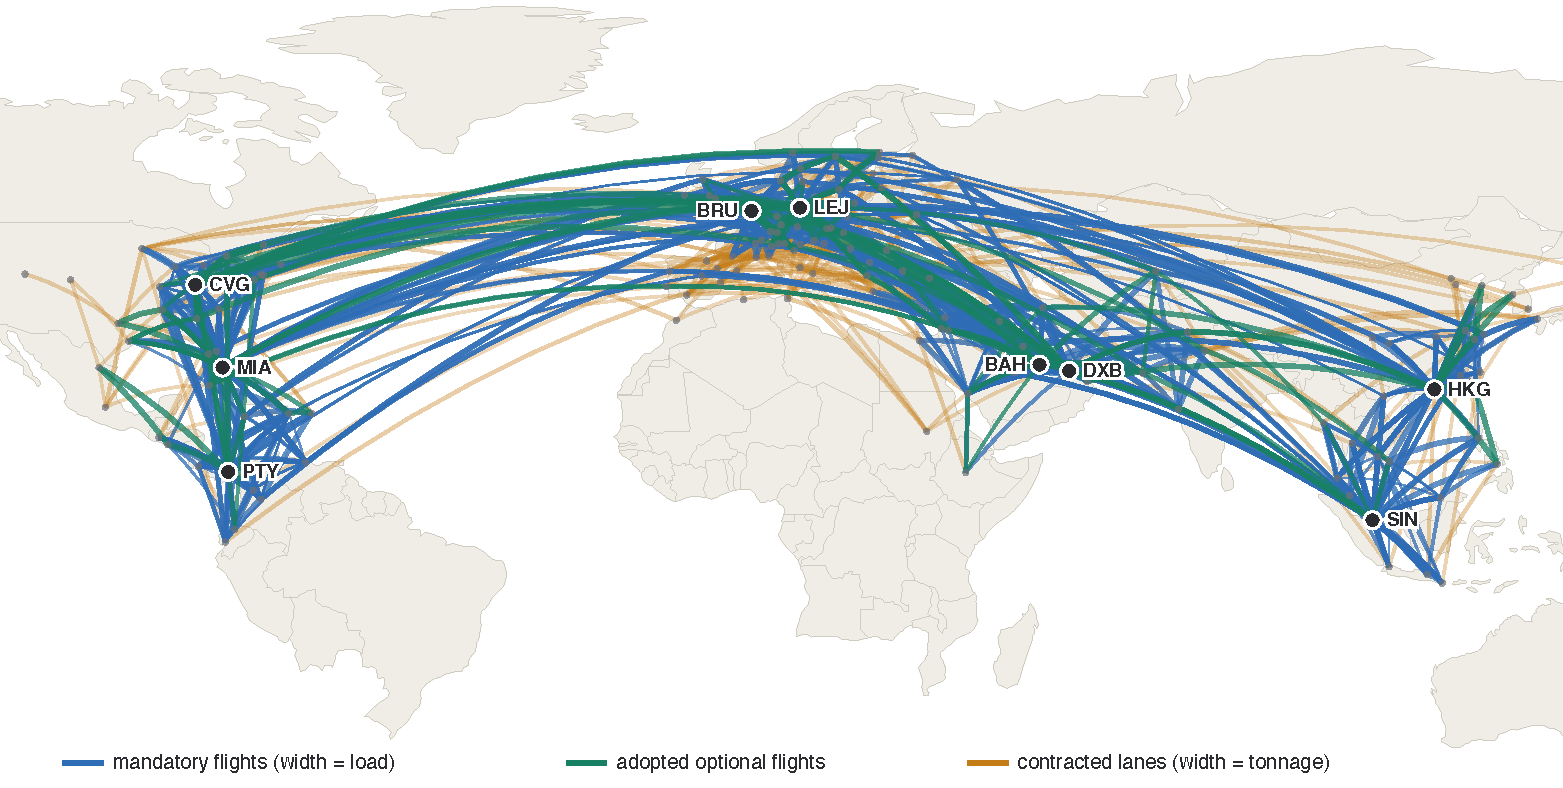
\includegraphics[width=\textwidth]{fig-map.pdf}
\caption{The best full-demand schedule on RLA-I-s1, drawn to scale. Blue:
mandatory flights (width $=$ load); green: adopted optional flights; amber,
underneath: the 250 heaviest \emph{contracted} lanes (width $=$ tonnage)
--- demand served by paid external carriers. The amber fans around the
hubs are the 46.6\,M contracting bill of Section~\ref{sec:results:pipeline}
made visible, and the target of the wave, relay and decomposition
experiments.}
\label{fig:map}
\end{figure}

\begin{table}[t]
\centering\small
\begin{tabular}{lr}
\toprule
airports / transfer hubs & 150 / 9 \\
fleets (aircraft) & 6 (154) \\
flights in base schedule (mandatory / optional) & 1{,}250 (625 / 625) \\
shipments (O\&D demands) & 29{,}819 \\
total demand & ${\sim}62.7$\,kt/week \\
service commitment & deliver-all (Section~\ref{sec:deliverall}) \\
\bottomrule
\end{tabular}
\caption{The integrator-scale instance RLA-I-s1 (synthetic, seed 1).}
\label{tab:instances}
\end{table}

\section{A deliver-all service model}\label{sec:deliverall}

Integrators do not cherry-pick profitable freight; a service commitment
means everything tendered is delivered, if necessary by a contracted
external carrier. We model this by (i) turning demand rows into equalities
and (ii) giving every shipment $od$ a \emph{contracted delivery column}
with objective coefficient $r_{od} - c^{\mathrm{rec}}_{od}$, upper bound
$d_{od}$, and a single nonzero entry in the demand row. The recourse tariff
is
\[
c^{\mathrm{rec}}_{od} \;=\; \mu \cdot \bigl( \delta_{od}\,v + \delta_{od}\,
\phi / W \bigr),
\]
with $\delta_{od}$ the great-circle distance, $v$ the average own variable
cost per tonne-km, $\phi$ the median own fixed cost per km, $W$ the largest
fleet payload, and $\mu=3$ throughout. Crucially, $v$ and $\phi$ are derived
from the \emph{mandatory} flights only: that set is identical in every model
variant of a design or decomposition run (optional candidates come and go),
so the tariff --- and hence the profit scale --- is stable across all
comparisons. An earlier version derived the tariff from all flights and
suffered a ${\sim}1\%$ per-round drift that silently invalidated
round-over-round comparisons.

Three consequences matter. Revenue becomes a constant, so the problem is a
cost minimization (own flying vs.\ contracting bill). Every selection of
flights is completable, so seeds, restricted sub-MIPs and decomposition
blocks are feasible by construction --- the entire pipeline of
Sections~\ref{sec:adoption} and~\ref{sec:regional} leans on this. And the
recourse coefficient caps the demand duals at the tariff, a free mild
stabilization of the master.

\section{Integer adoption at scale}\label{sec:adoption}

At integrator scale the practical failure is primal: branch-and-bound
explores 1--3 nodes within realistic budgets
(Section~\ref{sec:results:root}), so incumbents must come from elsewhere.
Our pipeline has four stages, each measured in isolation in
Table~\ref{tab:waterfall}.

\paragraph{(a) Greedy cover seed.} A constructive pass assigns every
mandatory flight to its lightest compatible fleet as balanced round trips
(inter-hub mirror pairs kept together), followed by an evaluated repair loop.
The seed is feasible but flowless: it earns no revenue (deliver-all:
everything is contracted).

\paragraph{(b) Seed flow loader.} After the root column generation, the
seed's selection is fixed in the master and \emph{one} warm LP optimizes
cargo flows over the column pool the pricers just generated. This is where
column generation pays its first dividend: the pool contains thousands of
priced itineraries, and one LP monetizes the skeleton in seconds. No new
pricing is needed.

\paragraph{(c) Escalating local-branching ball.} The primal heuristic solves
the restricted master MIP inside a Hamming ball of at most $k$ selection
flips around the incumbent \cite{fischetti2003}, escalating
$k \to 2k \to 4k$ (default $k=60$) while flat within a budget slice. The
incumbent is always feasible inside the ball, so the step is monotone; the
solver, not a hand-built neighborhood, chooses \emph{which} flips, which
keeps cross-network rotation rewirings reachable. An unrestricted
restricted-master MIP at this scale finds nothing in equal budget
(Table~\ref{tab:waterfall}); the ball turns the same budget into adopted
profit. On adoption, flows are re-monetized by one further warm LP.

\paragraph{(d) Promise vs.\ adoption.} Each design round logs the LP bound
uplift contributed by the current candidate batch (\emph{promise}) against
the integer profit actually adopted. This single observable separated two
hypotheses we could not otherwise distinguish --- ``the proposer generates
worthless candidates'' vs.\ ``the integer layer cannot digest them'' ---
and later diagnosed a genuine economic no (Section~\ref{sec:results:neg}).

\section{The autonomous design loop}\label{sec:design}

The base algorithm assumes a human writes the optional-flight candidate
list; this section removes that assumption without enumerating the slot
space. Each round, a proposer reads the previous solution's gaps ---
unroutable demand and capacity-crowded shipments, ranked by revenue at risk
--- and generates a batch from four classes:

\begin{itemize}
\item \emph{Hub round trips}, timed to stranded demand's availability
  windows: a pickup toward the nearest hub, a delivery from it, proposed as a
  coordinated pair when neither endpoint is itself a hub.
\item \emph{Direct point-to-point rotations}, sampled without replacement
  with probability proportional to proximity and to the pair's share of its
  origin's unserved volume --- close, locally dominant flows are the ones a
  direct can win.
\item \emph{Inter-hub trunk shuttles}, aimed at aggregate cross-hub tonnage
  after assigning every shipment's endpoints to their nearest hubs; these
  feed all multi-hub itineraries at once and are therefore exempt from zone
  filtering.
\item \emph{Premium external capacity} as a last resort, for pairs no
  own-fleet proposal reaches; the model books it only if the demand still
  pays at that price.
\end{itemize}

Batch quotas keep lower-priority classes from being starved on dense
instances, and deterministic keys (route plus departure bucket) deduplicate
against everything alive or recently evicted. The extended instance is then
re-solved with a warm-started column pool and the previous schedule seeded as
incumbent --- so a round can never return less than its predecessor ---
candidates are scored by whether they actually flew, and persistent
non-flyers are evicted, which keeps the \emph{active} model bounded while the
\emph{explored} candidate space grows without limit. Amnesty lets an evicted
candidate return some rounds later, since the network context changes as
accepted flights accumulate.

Two scale devices are toggleable: consolidation of tiny, far shipments into
hub-corridor pseudo demands during the rounds --- the final solve always runs
on the original demand, so delivered schedules and profits stay exact --- and
zone rotation of proposal targeting, so each hub cluster receives a full
batch and local synergies land in the same round. Algorithm~\ref{alg:design}
states the loop; full parameterization is in the repository's technical
report. One further class is a negative result we keep in the codebase,
disabled: \emph{hub waves}, coordinated feeder--trunk--distribution bundles
proposed as a set for the long tail of scattered small shipments. The
optimizer never adopted one (Section~\ref{sec:results:neg}).

\begin{algorithm}[t]\small
\SetKwInOut{Input}{input}\SetKwInOut{Output}{output}
\Input{base instance $I_0$; batch size $B$; per-round budget; eviction window
$\bar{e}$; flat-round limit $\bar{f}$}
\Output{best schedule found, and the instance it flies on}
$I \leftarrow I_0$;\quad $\sigma \leftarrow \textsc{GreedyCover}(I)$
  \tcp*{feasible, flowless seed}
$(\sigma,\Pi) \leftarrow \textsc{Solve}(I,\sigma,\emptyset)$
  \tcp*{$\Pi$: generated column pool}
$\sigma^\star \leftarrow \sigma$;\quad $\text{flat} \leftarrow 0$\;
\For{$r=1,2,\dots$ \KwSty{while} $\text{flat} < \bar{f}$}{
  $U \leftarrow$ unserved tonnage of $\sigma$ per shipment, ranked by revenue at
    risk\;
  $C \leftarrow \textsc{Propose}(I,U,B,\text{zone}(r),\text{blocked keys})$
    \tcp*{hub / direct / trunk / external}
  \lIf{$C = \emptyset$}{\KwSty{continue}, or stop after a full empty cycle}
  $(\sigma^{+},\Pi) \leftarrow \textsc{Solve}(I \cup C,\ \sigma,\ \Pi)$
    \tcp*{seeded incumbent, warm columns}
  \lIf{$\sigma^{+} = \bot$}{drop $C$, prune $\Pi$ to $I$'s ids,
    \KwSty{continue}}
  mark each $c \in C$ flown in $\sigma^{+}$; evict candidates unflown for
    $\bar{e}$ consecutive rounds\;
  $I \leftarrow (I \cup C) \setminus \text{evicted}$;\quad remap $\Pi$ and
    $\sigma^{+}$ to the new ids\;
  \KwSty{log} $\bigl(\text{bound uplift of } C,\ \text{profit adopted}\bigr)$
    \tcp*{promise vs.\ adoption}
  \eIf{$\mathrm{profit}(\sigma^{+}) > \mathrm{profit}(\sigma^{\star})$}{
    $\sigma^{\star} \leftarrow \sigma^{+}$;\quad $\text{flat} \leftarrow 0$\;
  }{
    $\text{flat} \leftarrow \text{flat} + 1$\;
  }
  $\sigma \leftarrow \sigma^{+}$\;
}
\Return{$\textsc{ExactFinal}(\sigma^{\star})$, solved on the full,
unconsolidated demand}
\caption{Autonomous design loop (Section~\ref{sec:design}).}
\label{alg:design}
\end{algorithm}

\section{Geographic fix-and-optimize with exact gateway windows}
\label{sec:regional}

Motivated by the observation that block-sized models adopt improvements in
seconds while the whole-network master adopts nothing
(Section~\ref{sec:results:regional}), we decompose the planet: hub clusters
(hubs within 3{,}000\,km) define regions; every airport joins its nearest
hub's region.

\paragraph{Blocks.} A block re-optimizes one region against a frozen world.
Re-decidable (\emph{kept}) flights are those with every leg inside the
region, minus three repair classes computed to a fixpoint: (i)
\emph{balance repair} --- the kept \emph{selected} strings must balance
arrivals and departures per (fleet, airport), or neither side of the
partition assembles into rotations; unbalanced one-way strings (typically a
multi-stop trunk whose mirror has an en-route stop in a third region) are
frozen one at a time, so the cascade follows the unbalanced chain and stops;
(ii) flows whose path crosses the region more than once, and (iii)
degenerate cuts (a loop entering and leaving at the same airport), whose
flights are frozen because the merge splices exactly one regional segment
per donated flow.

\paragraph{Exact windows.} Cross-boundary cargo is truncated at its gateway
with windows read from the \emph{frozen timetable}, not estimated: an
outbound segment must end before its frozen onward connection departs minus
the gateway transfer time; an inbound segment becomes available when its
frozen feeder lands plus transfer. Cargo handling at true origins and
destinations is encoded into the windows so gateway hand-offs do not pay it
twice. Consequently a time-feasible block solution \emph{splices} back into
a time-feasible global schedule by construction. Shipments with both
endpoints inside the region enter whole; under deliver-all their contracted
remainder rides along, so every block is feasible from its seed.

\paragraph{Fleet slice.} The block's fleet budget is
$\mathrm{count} - \mathrm{used}(\mathrm{all}) +
\mathrm{used}(\mathrm{kept})$, computed by assembling the kept side alone
(possible after balance repair). Splitting mixed rotation chains can cost a
rounding aircraft per fragment that no a-priori budget foresees; instead of
estimating it, the cycle \emph{learns} it: a merged block that fails the
global fleet-size check by $e_k$ aircraft teaches its block a budget
reduction of $e_k$ for the next visit.

\paragraph{Monotone merge.} A block solution is spliced into the global
schedule (frozen strings and flows kept; donated segments replaced;
sub-contracted remainders fall back to global end-to-end contracting) and
accepted \emph{only if} the independently verified global profit improves.
The cycle can therefore never lose ground (Proposition~\ref{prop:monotone}).

Algorithm~\ref{alg:block} states block construction and the cycle. Two
properties make the scheme safe; both are immediate, and we state them
because they are what a reader must be able to check.

\begin{proposition}[Splice feasibility]\label{prop:splice}
Let $\sigma$ be a globally feasible schedule and let a block be built as in
Algorithm~\ref{alg:block}. If $\sigma_B$ is a feasible solution of the block
instance, then every shipment of the merged schedule remains time-feasible:
each donated segment is replaced by one whose elapsed time lies in
$[\alpha,\beta]$, where $\alpha$ is the arrival of the frozen feeder plus the
gateway transfer time and $\beta$ the departure of the frozen onward
connection minus it, both read from $\sigma$'s unchanged timetable.
\end{proposition}

\begin{proof}
Frozen flights keep their departure and arrival times, so $\alpha$ and $\beta$
are unaffected by anything the block decides. A block shipment's release and
deadline are set to exactly $\alpha$ and $\beta$ by construction, and
$\sigma_B$ respects them; splicing therefore preserves every connection time
on both sides of the gateway. Shipments crossing the region more than once,
and degenerate cuts, are excluded from donation by the partition step, so
each donated path receives exactly one replacement segment. \qed
\end{proof}

\begin{proposition}[Monotonicity]\label{prop:monotone}
The regional cycle never decreases the global objective, and every schedule
it returns is feasible for the original instance.
\end{proposition}

\begin{proof}
A merged schedule is adopted only if it passes the independent feasibility
check and strictly improves the globally recomputed objective; otherwise the
incumbent is kept unchanged. Both statements are therefore loop invariants,
and hold of the returned schedule in particular. \qed
\end{proof}

Proposition~\ref{prop:splice} is what the construction \emph{intends};
Proposition~\ref{prop:monotone} is what the implementation \emph{guarantees}
even when that intent is violated by a defect. Keeping both earned its
keep: during development the guard rejected four distinct merge defects
(Section~\ref{sec:results:regional}) without ever admitting a corrupted
schedule.

\paragraph{Pairwise relay.} Optionally, after the single-region passes of
each cycle, \emph{pair} passes run on region unions ordered by open
cross-tonnage. A cross-region shipment enters a pair block whole, with
exact windows; feeder, trunk and distribution are decided in one model,
avoiding any cross-pass ledger or estimated hand-off times.

\begin{algorithm}[t]\small
\SetKwInOut{Input}{input}\SetKwInOut{Output}{output}
\Input{instance $I$, incumbent $\sigma$, regions $\mathcal{R}$, per-block and
total budgets}
\Output{a schedule at least as good as $\sigma$ (Proposition~\ref{prop:monotone})}
$\text{shave} \leftarrow \mathbf{0}$
  \tcp*{learned fleet corrections, per block}
\ForEach{cycle, \KwSty{and} pass $R$ over $\mathcal{R}$ then over
  cross-loaded region pairs}{
  \tcc{partition: which flights may this block re-decide?}
  $\mathcal{K} \leftarrow \{f \in F : \text{every leg of } f
    \text{ lies inside } R\}$\;
  \Repeat{$\mathcal{K}$ unchanged}{
    \ForEach{$(\text{fleet},\text{airport})$ with unbalanced kept selected
      strings}{freeze one contributing one-way string\;}
    freeze the flights of flows crossing $R$ more than once, and of
      degenerate cuts\;
  }
  \lIf{$\mathcal{K}$ contains no cargo flight}{\KwSty{continue}}
  \tcc{demand: exact windows read from the frozen timetable}
  \ForEach{shipment $q$}{
    \uIf{both endpoints of $q$ lie in $R$}{
      add $q$ whole, window shrunk by handling at both ends\;
    }\ElseIf{$\sigma$ routes $q$ through $\mathcal{K}$ on exactly one run
      $[s,e]$}{
      add a sub-shipment for that run, with release $\alpha$ and deadline
      $\beta$ as in Proposition~\ref{prop:splice}\;
    }
  }
  $n^{B}_k \leftarrow n_k - \text{used}_k(\sigma) + \text{used}_k(\mathcal{K})
    - \text{shave}_k[R]$ \tcp*{block fleet slice}
  seed $\leftarrow$ kept strings and their flows; remainder contracted\;
  $\sigma_B \leftarrow \textsc{Solve}(\text{block},\ \text{seed})$;\quad
  $\sigma' \leftarrow \textsc{Merge}(\sigma,\sigma_B)$\;
  \eIf{$\sigma'$ feasible \KwSty{and}
    $\mathrm{profit}(\sigma') > \mathrm{profit}(\sigma)$}{
    $\sigma \leftarrow \sigma'$\;
  }{
    \lIf{$\sigma'$ exceeds fleet $k$ by $e_k$ aircraft}{
      $\text{shave}_k[R] \leftarrow \max(\text{shave}_k[R],\, e_k)$}
  }
}
\Return{$\sigma$}
\caption{Geographic fix-and-optimize cycle (Section~\ref{sec:regional}).}
\label{alg:block}
\end{algorithm}

\section{Engineering for honest measurement}\label{sec:engineering}

\paragraph{Parallel pricing, bit-identical.} Each pricing iteration asks one
independent shortest-path question per shipment against the same duals. The
sweep runs one shipment per core and collects results in shipment order, so
its output is bit-identical to the sequential sweep (asserted by test and
verified in production runs: identical column counts and bounds). The
per-destination A${}^{*}$ bounds --- the only lazily built shared state ---
are prewarmed one Dijkstra pair per core. The servability probes of the
design loop parallelize the same way with thread-local dual vectors.

\paragraph{Mispricing-safe dual smoothing.} Optionally, pricers see
$\alpha \cdot \mathrm{center} + (1-\alpha)\cdot \mathrm{duals}$
\cite{wentges1997,dumerle1999} ($\alpha=0.7$). Two safeguards keep
exactness: a smoothed pass that finds no columns triggers a re-price with
the true duals before any conclusion, and validity-critical bounds are
computed from true-dual passes only. A test asserts that the stabilized
root converges to the same LP value as the plain one. We report no
performance numbers for smoothing: it is implemented, verified and off by
default, and its evaluation is deliberately left to the multi-seed battery
--- we flag this to avoid claiming a benefit we have not measured.

\paragraph{Bounds under truncation.} Hard per-round budgets are made
mathematically legal by a Farley-type bound \cite{farley1990}: on
interruption the tightest valid bound seen across full pricing passes is
returned, each computed as the RMP value plus the most optimistic
contribution of \emph{missing} columns. A membership filter is essential in
practice: pricers legitimately return columns already in the master
(nonbasic at bounds, positive reported reduced cost); counting them
produces absurd bounds. Only columns not yet in the master contribute.

\paragraph{Cost visibility.} Every colgen iteration reports its breakdown
(pricing / column loading / LP re-solve seconds). This 20-line addition
settled in minutes a question we had been guessing at for days
(Section~\ref{sec:results:parallel}).

\section{Computational results}\label{sec:results}

\emph{Protocol and disclosure.} All numbers below are from single runs on
one machine (Apple Silicon, 10 cores; CPLEX 22.2 as LP/MIP backend, HiGHS
as fallback), on instance RLA-I-s1 unless stated. They are exploratory:
no variance estimates, one seed. We report them because their margins are
large and their patterns repeated across the campaign; the multi-seed
battery over all instance families is the declared next step. All runs are
reproducible from the public repository (deterministic seeds; every
figure's raw log is committed).

\subsection{Where the branch-and-bound tree earns its keep}
\label{sec:results:tree}

Before reporting what fails, we report where the base method works.
Table~\ref{tab:tree} solves one instance of each family with the plain
procedure (column generation, cuts, branching, restricted-master heuristic;
no matheuristic layer) under a short budget.

\begin{table}[t]
\centering\small
\begin{tabular}{lrrrrrr}
\toprule
instance & shipments & flights & nodes & gap & time (s) & termination \\
\midrule
RC-I  &    800 &   100 &      3 & 0.00\% &   0.1 & tree exhausted \\
IC-I  &  3{,}500 &   310 &      1 & 0.00\% &   0.4 & tree exhausted \\
MI-I  &  4{,}000 &   400 & 13{,}698 & 1.66\% & 180.0 & time limit \\
EX-I  &  6{,}000 &   900 &  2{,}867 & 0.73\% & 180.0 & time limit \\
GI-I  &  9{,}000 & 1{,}250 &      1 & 0.43\% &  97.6 & gap target \\
\midrule
RLA-I$^{\dagger}$ & 29{,}819 & 1{,}250 & 1--3 & 9.9\% & 5{,}400 & no improvement \\
\bottomrule
\end{tabular}
\caption{The base branch-and-price-and-cut across instance families, short
budgets, no matheuristic layer. $^{\dagger}$RLA is the deliver-all
integrator instance of Table~\ref{tab:instances}, run inside the design
pipeline (Section~\ref{sec:results:root}); it differs from the others in
more than size.}
\label{tab:tree}
\end{table}

Three regimes are visible. On the small families the LP relaxation is
integral or nearly so and the tree closes in milliseconds. In the middle
(MI, EX) the relaxation is genuinely fractional and the tree does the work
it was designed for --- thousands of nodes, gaps under 2\%. At GI scale
(9{,}000 shipments, 1{,}250 flights) the root relaxation is already good
enough that \emph{one} node reaches a 0.43\% gap in 98 seconds: the tree is
not failing there, it is unnecessary. Only at RLA scale does the picture
change qualitatively.

We stress what this table does \emph{not} establish. RLA differs from GI in
more than shipment count --- it carries the deliver-all service commitment,
gravity demand over 60\% of station pairs, nine hubs instead of four, and
weekly lane recurrence --- so these measurements locate the breakdown
between the two families without isolating its cause. A controlled scaling
series over one family is the experiment that would, and it is not yet run.

\subsection{The whole-network integer layer stalls}\label{sec:results:root}

At RLA scale the regime of Table~\ref{tab:tree} changes. From a shared
incumbent at 139.7--139.8\,M (produced by cover seed + loader), the
whole-network solver --- warm-started column pool, seeded
incumbent, escalating ball, 90-minute budget --- produced \emph{zero}
incumbent improvements, twice (independent runs at 1{,}800\,s and
5{,}400\,s produced the same $+0$). Branch-and-bound explored 1--3 nodes.
This is the phenomenon the rest of the paper responds to: at this scale the
exact tree is vestigial and even ball-restricted sub-MIPs drown in the full
master's LP.

\subsection{The adoption pipeline}\label{sec:results:pipeline}

Table~\ref{tab:waterfall} and Figure~\ref{fig:waterfall} show the round-0 waterfall on the consolidated
design model (25{,}451 demands after tiny-far consolidation). Each stage is
enabled on top of the previous.

\begin{table}[t]
\centering\small
\begin{tabular}{lrr}
\toprule
stage & profit (M) & increment \\
\midrule
greedy cover seed (all demand contracted) & 129.9 & --- \\
+ seed flow loader (one warm LP over the pool) & 139.6 & $+9.7$ \\
+ local-branching ball $k{=}60$ & 142.3 & $+2.7$ \\
+ adoption re-monetization (one warm LP) & 143.3 / 143.5 & $+1.0$ \\
\midrule
unrestricted restricted-master MIP, same budget & 139.6 & $+0.0$ \\
\bottomrule
\end{tabular}
\caption{Round-0 incumbent waterfall on RLA-I-s1 (consolidated model,
deliver-all). The re-monetization column shows two
independent runs. The last row is the ablation: without the ball, the same
heuristic budget adopts nothing.}
\label{tab:waterfall}
\end{table}

\begin{figure}[t]
\centering
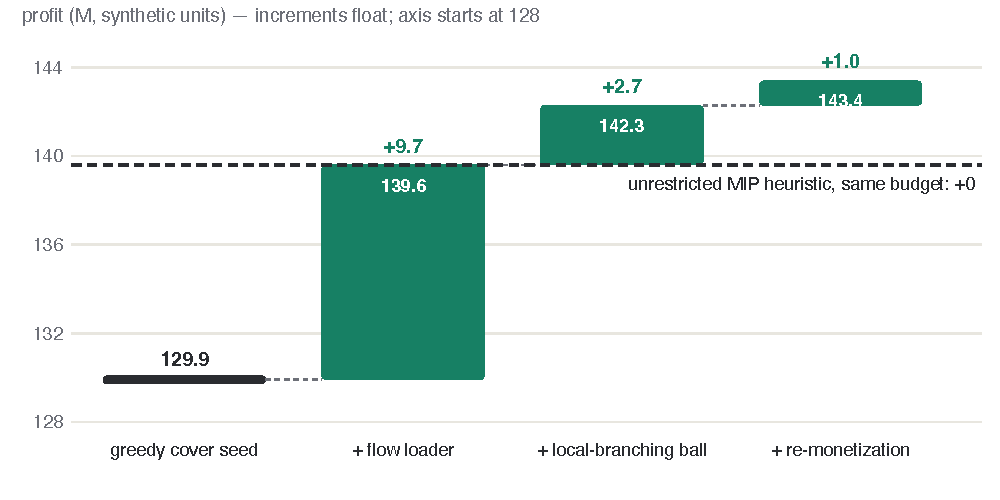
\includegraphics[width=.8\textwidth]{fig-waterfall.pdf}
\caption{The adoption pipeline of Section~\ref{sec:adoption} as a
waterfall (data of Table~\ref{tab:waterfall}). Green segments are the
increments each stage adds on top of the previous; the dashed line is the
ablation --- the unrestricted restricted-master MIP, given the same budget
as the ball, never leaves the loader's level.}
\label{fig:waterfall}
\end{figure}

The best full-demand schedule obtained by the design pipeline alone reaches
142.8\,M at a 9.9\% gap against the run's dual-bound estimate (the
certification caveat, Limitation~(viii), applies); in it, 22{,}011 of 29{,}819 shipments
(46.0\,kt, a 46.6\,M bill) are contracted and only 58 of 154 aircraft fly.
That anatomy --- a long tail of ${\sim}2$-tonne shipments scattered over
${\sim}150$ stations, the amber fans of Figure~\ref{fig:map} --- motivates both the wave experiment (negative,
below) and the decomposition (positive, next).

\subsection{Geographic decomposition}\label{sec:results:regional}

A/B protocol: one shared base incumbent, then the same additional budget
spent either (A) continuing the whole-network solve or (B) running the
regional cycle. Table~\ref{tab:regional} summarizes four consecutive runs
(two clean A/Bs plus two earlier runs whose arm B was invalidated by merge
bugs --- in \emph{every} run, including the buggy ones, the global
feasibility guard held: no corrupted schedule was ever accepted).

\begin{table}[t]
\centering\small
\begin{tabular}{lrrl}
\toprule
arm & budget & gain & note \\
\midrule
A: whole-network continuation & 1{,}800\,s & $+0$ & \\
A: whole-network continuation & 5{,}400\,s & $+0$ & independent repeat \\
B: regional cycle & 900\,s & $+5.03$\,M & 6 accepted blocks, then flat \\
B: regional cycle (learned fleet shave) & 1{,}800\,s & $+3.96$\,M &
includes learning visits \\
\bottomrule
\end{tabular}
\caption{Whole-network vs.\ regional split from a shared incumbent
(RLA-I-s1, full 29{,}819-shipment demand). Blocks of 200--350 flights
adopt improvements in 4--50 seconds each.}
\label{tab:regional}
\end{table}

\begin{figure}[t]
\centering
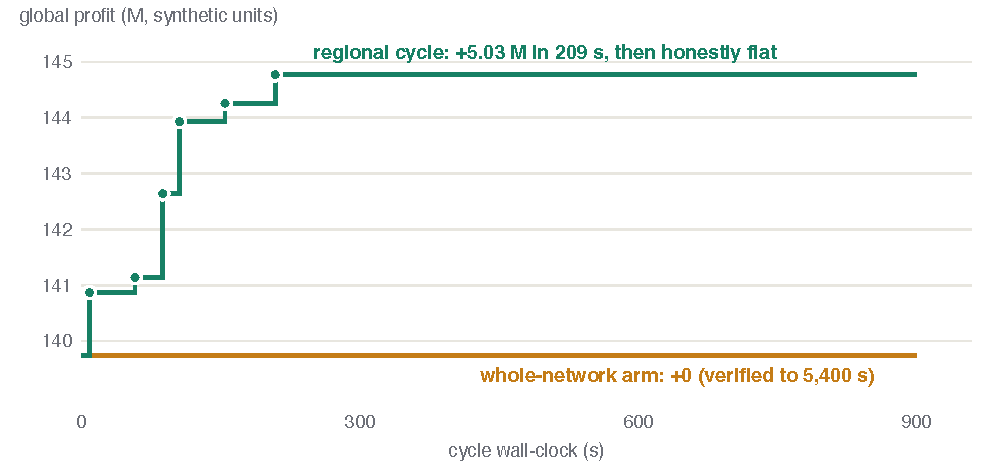
\includegraphics[width=.8\textwidth]{fig-regional.pdf}
\caption{The clean A/B of Table~\ref{tab:regional}, over the cycle clock.
Each dot is an accepted block merge (globally verified); the plateau after
209\,s is the cycle reporting flat blocks rather than manufacturing noise.
The whole-network arm, from the same incumbent, adopts nothing in
5{,}400\,s.}
\label{fig:regional}
\end{figure}

The mechanism, not just the outcome, matches the diagnosis: all four
regions adopt on their first visit (from $+0.26$\,M to $+1.5$\,M each, in
9--50\,s of block time), improvements shrink on the second cycle, and the
cycle then honestly reports flat blocks until the budget closes. The best
full-demand schedule of the campaign (144.8\,M) came from a 5-minute base
solve plus a 15-minute regional cycle.

\subsection{Negative results}\label{sec:results:neg}

\emph{Hub waves.} A fifth candidate class proposed coordinated
feeder--trunk--distribution bundles per (hub corridor, day), with
chain-consistent times and honestly windowed tonnage. Over 20 design rounds
(6{,}000 candidates, waves included at 30\% quota), \emph{zero} were
adopted, and the LP promise of candidate batches decayed from $+4.4$\,M
(round 1) to ${\sim}0$ (round 3 on). \emph{Pair relay.} The pairwise
passes of Section~\ref{sec:regional} ran clean (no crashes, all merges
verified) and adopted nothing at $\mu=3$. \emph{Interpretation.} Three
independent probes --- waves, promise decay, pairs --- agree: at triple own
economics, the scattered cross-region tail is genuinely cheaper to
contract than to fly. This is a statement about the instance's economics,
not about the algorithms; both mechanisms remain in the code, disabled by
default, for cheaper-recourse or larger-scale settings.

\emph{LP method.} On the colgen master ($>40$k columns), CPLEX sifting ---
nominally suited to column-heavy LPs --- measured $2$--$3\times$
\emph{slower} per re-solve (49--114\,s) than warm-started dual simplex
(18--44\,s). The advantage of basis reuse across colgen iterations is
well known; the value here is quantifying it for this master, since it
rules out a drop-in remedy for the LP bottleneck of
Section~\ref{sec:results:parallel}.

\subsection{Parallel pricing and the next bottleneck}
\label{sec:results:parallel}

Parallelizing the pricing sweep cut it from ${\sim}25$\,s to
0.4--1.0\,s per iteration (identical columns and bounds), but end-to-end
root time improved only ${\sim}15\%$ (156\,s $\to$ 133\,s for six
iterations). The per-iteration breakdown explains it: pricing 1.0\,s,
column loading 0.1\,s, master LP re-solve 18--44\,s and growing with the
column count. Amdahl's ledger is now unambiguous: the master LP is the
next bottleneck, and the natural lever is column deletion (keeping the
master lean) rather than a faster pricer. Dual smoothing also gains value
from this shift: every avoided iteration now saves a full LP re-solve.

\section{Limitations}\label{sec:limits}

(i) Headline results are single-seed, single-machine, one instance family
at scale; margins are large but variances are unmeasured. (ii) All
instances are synthetic; parameters (costs, demands, fleets, curfews,
payload-range curves) are AI-estimated for plausibility and calibrated in
scale --- not in detail --- to \cite{derigs2013}; no real airline data is
used or implied. (iii) Comparability with \cite{derigs2013} is qualitative
only: their instances and code were not published, so our reimplementation
of their generators matches parameters, not files. (iv) There is no
external baseline yet (e.g., a direct arc-flow MIP under equal budget);
``better than our own previous configuration'' is the only comparison this
preprint supports. (v) The design loop is greedy across rounds; inner
solves carry valid bounds, but no global optimality claim spans rounds.
(vi) The breakdown of Table~\ref{tab:tree} is located between two instance
families that differ in several factors at once; a controlled scaling series
within one family is needed to attribute it to size.
(vii) We do not compare against the concurrent model of \cite{zhu2026}: the
horizons differ (single night vs.\ periodic week) and neither instance set
is expressible in the other's formulation without changing the problem, so a
head-to-head would compare problems rather than methods.
(viii) A post-campaign code audit (September 2026) found and fixed two
defects that affect the reported numbers, not the mechanisms. First,
design-round instance rebuilds silently dropped the cargo-handling time
(30 to 0 minutes), relaxing connection windows for the designed networks
relative to the correctly handled baseline; the design-uplift margins are
therefore optimistic until re-measured. Second, the dual bound combined a
label-capped path pricer, which can miss an od's best path, with a
fleet-size string aggregation that strings crossing no fleet-count time
escape, so pre-fix gaps --- including the 9.9\% above --- are estimates,
not certificates. The solver now recomputes the Farley bound from an
uncapped confirmation pass with a flight-cover string aggregation and
stamps every run with a certification flag; the multi-seed battery of the
road map will run entirely on the fixed solver.

\section{Conclusions and road map}\label{sec:conclusions}

At integrator scale, the exact tree of B\&P\&C contributes almost nothing,
but the column-generation engine remains the value chain's spine: every
profitable move in our campaign flowed through priced columns, warm LPs
over them, or dual signals derived from them. The productive question is
not ``exact or heuristic'' but \emph{where each layer earns its keep}:
LP/colgen for columns, prices and certificates; local branching for
integer moves the full master cannot digest; geographic fix-and-optimize
for turning block-sized tractability into global, verified, monotone
progress.

Road map, in order: (1) the multi-seed battery over all instance families
with component ablations; (2) an arc-flow MIP baseline under equal budget;
(3) column deletion for the master LP; (4) deeper trees inside regional
blocks, where nodes cost seconds; (5) any form of real-data validation,
which would upgrade every claim in this paper.

\section*{Reproducibility and AI disclosure}

The complete implementation (solver, generators, web workbench, 124
verification tests) and all instance generators are public in the
accompanying repository; instances and every run output are regenerated
deterministically from their integer seeds by the commands documented
there --- raw logs themselves are not versioned. This project was developed with substantial
assistance from an AI coding agent (Anthropic Claude), including code,
instance parameter estimation, experiment execution and the drafting of
this manuscript; all algorithmic decisions, measurements and claims were
verified by the reproducible pipeline above, and the human author reviewed
and takes responsibility for the content. Airline names and data are
fictional.

\begin{thebibliography}{19}\small

\bibitem{derigs2013} Derigs, U., Friederichs, S.:
Air cargo scheduling: integrated models and solution procedures.
OR Spectrum 35, 325--362 (2013).

\bibitem{barnhart1998} Barnhart, C., Johnson, E.L., Nemhauser, G.L.,
Savelsbergh, M.W.P., Vance, P.H.: Branch-and-price: column generation for
solving huge integer programs. Operations Research 46(3), 316--329 (1998).

\bibitem{lubbecke2005} L\"ubbecke, M.E., Desrosiers, J.: Selected topics in
column generation. Operations Research 53(6), 1007--1023 (2005).

\bibitem{desaulniers2005} Desaulniers, G., Desrosiers, J., Solomon, M.M.
(eds.): Column Generation. Springer (2005).

\bibitem{fischetti2003} Fischetti, M., Lodi, A.: Local branching.
Mathematical Programming 98, 23--47 (2003).

\bibitem{danna2005} Danna, E., Rothberg, E., Le Pape, C.: Exploring
relaxation induced neighborhoods to improve MIP solutions. Mathematical
Programming 102, 71--90 (2005).

\bibitem{wentges1997} Wentges, P.: Weighted Dantzig--Wolfe decomposition
for linear mixed-integer programming. International Transactions in
Operational Research 4(2), 151--162 (1997).

\bibitem{dumerle1999} du Merle, O., Villeneuve, D., Desrosiers, J., Hansen,
P.: Stabilized column generation. Discrete Mathematics 194, 229--237
(1999).

\bibitem{farley1990} Farley, A.A.: A note on bounding a class of linear
programming problems, including cutting stock problems. Operations
Research 38(5), 922--923 (1990).

\bibitem{shaw1998} Shaw, P.: Using constraint programming and local search
methods to solve vehicle routing problems. In: Principles and Practice of
Constraint Programming (CP), 417--431 (1998).

\bibitem{ropke2006} Ropke, S., Pisinger, D.: An adaptive large neighborhood
search heuristic for the pickup and delivery problem with time windows.
Transportation Science 40(4), 455--472 (2006).

\bibitem{helber2010} Helber, S., Sahling, F.: A fix-and-optimize approach
for the multi-level capacitated lot sizing problem. International Journal
of Production Economics 123(2), 247--256 (2010).

\bibitem{archetti2014} Archetti, C., Speranza, M.G.: A survey on
matheuristics for routing problems. EURO Journal on Computational
Optimization 2(4), 223--246 (2014).

\bibitem{fischetti2018} Fischetti, M., Fischetti, M.: Matheuristics. In:
Mart\'{\i}, R., Pardalos, P.M., Resende, M.G.C. (eds.) Handbook of
Heuristics. Springer (2018).

\bibitem{crainic2000} Crainic, T.G.: Service network design in freight
transportation. European Journal of Operational Research 122(2), 272--288
(2000).

\bibitem{feng2015} Feng, B., Li, Y., Shen, Z.-J.M.: Air cargo operations:
literature review and comparison with practices. Transportation Research
Part C: Emerging Technologies 56, 263--280 (2015).

\bibitem{zhu2026} Zhu, L., Belieres, S., Hewitt, M., Wu, L.: Joint fleet
scheduling and cargo flow allocation for air cargo services. Transportation
Research Part B: Methodological 209, 103469 (2026).

\bibitem{derigs2009} Derigs, U., Friederichs, S., Sch\"afer, S.: A new
approach for air cargo network planning. Transportation Science 43(3),
370--380 (2009).

\bibitem{xiao2022} Xiao, F., Guo, S., Huang, L., Huang, L., Liang, Z.:
Integrated aircraft tail assignment and cargo routing problem with through
cargo consideration. Transportation Research Part B: Methodological 162,
328--351 (2022).

\bibitem{yildiz2022} Y{\i}ld{\i}z, B., Savelsbergh, M.: Optimizing package
express operations in China. European Journal of Operational Research 300(1),
320--335 (2022).

\bibitem{zheng2023} Zheng, H., Sun, H., Zhu, S., Kang, L., Wu, J.: Air cargo
network planning and scheduling problem with minimum stay time: a
matrix-based ALNS heuristic. Transportation Research Part C: Emerging
Technologies 156, 104307 (2023).

\bibitem{huang2023} Huang, L., Xiao, F., Zhou, J., Duan, Z., Zhang, H.,
Liang, Z.: A machine learning based column-and-row generation approach for
integrated air cargo recovery problem. Transportation Research Part B:
Methodological 178, 102846 (2023).

\bibitem{brandt2019} Brandt, F., Nickel, S.: The air cargo load planning
problem --- a consolidated problem definition and literature review.
European Journal of Operational Research 275(2), 399--410 (2019).

\bibitem{feillet2010} Feillet, D.: A tutorial on column generation and
branch-and-price for vehicle routing problems. 4OR 8(4), 407--424 (2010).

\bibitem{huangfu2018} Huangfu, Q., Hall, J.A.J.: Parallelizing the dual
revised simplex method. Mathematical Programming Computation 10(1), 119--142
(2018).

\end{thebibliography}

\end{document}
